\suppressfloats[t]
\section{Experimental Configuration}
\label{app:configuration}

\paragraph{Supply-chain environment and learner.}
The six-node \texttt{NetworkManagement-v1} network has 30-period episodes. Node 1 is scripted to order
20 units per period, split equally across its action entries; nodes 2--6 are controlled by one
parameter-shared PPO policy. Every trainable node's lane receives the same full or-gym observation of the
network state, with no agent identifier; actions are padded to the largest per-node action dimension, and each
node uses its leading entries, so under deterministic evaluation all five nodes receive the same action
vector. PPO uses Stable-Baselines3 2.8.0 with \texttt{n\_steps} $=128$, minibatch size 256, ten
optimization epochs, learning rate $3\times10^{-4}$, discount $0.99$, GAE coefficient $0.95$, policy
clip $0.2$, value-loss coefficient $0.5$, zero entropy coefficient, normalized minibatch advantages,
separate actor and critic MLPs of width 64, one Adam optimizer with SB3's implicit $\epsilon=10^{-5}$,
and global gradient max-norm $0.5$. Training is CPU-only and single-threaded, with an explicit simulator
random stream per environment.

\paragraph{Budget arithmetic.}
Budgets count requested agent transitions. Five lanes and 128-step rollouts add 640 transitions per
rollout, and training stops at the first completed rollout at or beyond the request: 300k requested
transitions execute 300,160 (469 rollouts), and each 150k checkpoint is evaluated at the first rollout
boundary after it. One agent transition is one node's step, so 300,160 transitions are 60,032 joint
environment periods (about 2,001 episodes).

\paragraph{Reward, reference point and controls.}
Each agent receives $x_i(w)=(1-w)r_i^{\mathrm{local}}+wr^{\mathrm{global}}$ before any transform. The
linear condition uses $v(x)=x$; curvature-only uses $\phi(x)=\operatorname{sign}(x)|x|^{.88}$; the
loss-multiplier condition uses $v_\lambda(x)=\phi(x)$ for $x\ge0$ and $\lambda\phi(x)$ for $x<0$. E1 and
E2 use the reference $z_0=-2.6281398333$, fixed before any of their runs as the pooled mean of raw
blended rewards from 40 untreated curvature-only calibration policies, with 7,500 samples at each of
the eight E1 mixture cells (60,000 samples). With $u=x-z_0$ and
$s_{\mathrm{in}}=1$, the arms are B$=\phi(u)$ ($s_{\mathrm{out}}=1$), A$=v_7(u)$ ($s_{\mathrm{out}}=1$),
S$=7\phi(u)$ ($s_{\mathrm{out}}=1/7$) and R$=3.451\,\phi(u)$ ($s_{\mathrm{out}}=1/3.451$, where 3.451 is
A's pooled transformed-reward RMS divided by B's in the earlier direct control). E3 uses reference zero.

\paragraph{Optimizer interventions.}
\texttt{separate\_no\_clip} builds two Adam optimizers with the default settings, one over the actor
parameters (policy MLP, action head, log-standard-deviation) and one over the critic parameters (value
MLP and head), applies the unchanged PPO loss, and skips gradient clipping; execution aborts if any
trainable parameter is shared. \texttt{VecNormalize} divides rewards by the running standard deviation of
discounted returns ($\gamma=0.99$, $\epsilon=10^{-8}$, reward clip 10, no observation normalization). E2
passes \texttt{optimizer\_kwargs=\{eps: 1e-8\}}. E6's \texttt{groupwise\_clip} keeps one Adam optimizer and
clips the actor and critic gradients to norm 0.5 separately; E6 also records, at every optimizer step and
for each parameter group, the post-clip gradient norm and the norm of the parameter change, by copying the
parameters before the step. Every run logs per-minibatch actor, critic and total
gradient norms before and after the clipping step.

\paragraph{Labels.}
The supply-chain label is $\mathbf{1}[\bar S<10\wedge\bar\pi\le-127.1]$, with $\bar S$ the mean over
nodes 2--6 of the deterministic base-stock target $250(a_1+1)$ at the reset of evaluation seed $10s$,
and $\bar\pi$ the ten-episode mean total profit on seeds $10s,\ldots,10s+9$. The LBF label is native
team return below 0.626 over ten deterministic episodes on seeds $10s,\ldots,10s+9$; the native return
excludes the effort cost.

\paragraph{LBF learner.}
MAPPO uses SB3 PPO with a centralized-critic policy: the actor's features come from the agent's own
observation and the critic's from the concatenated global state (feature width 128; actor heads
$[64,64]$, critic heads $[128,128]$), eight parallel environment copies, \texttt{n\_steps} $=256$,
minibatch 512, entropy coefficient 0.01, and \texttt{lbforaging} 2.0.0. In a check at 100k timesteps
on one cell and seed, the global-clip runner reproduced the legacy LBF runner's team return exactly.

\section{Boundary Estimation and Diagnostics}
\label{app:estimation}

For each fixed configuration we fit $P(Y=1\mid w)=\sigma(b_0+b_1w)$ by Firth logistic regression and
report $w_{50}=-b_0/b_1$. A point estimate is reported only with an identified nonzero slope; observed
proportions are inspected separately for adjacent cells bracketing $.5$. Confidence intervals use 2,000
percentile-bootstrap draws of complete training-seed blocks (multinomial weights over the ten seeds;
random seed 20261015 for E1--E8; E8's fresh-seed cohort uses the same weights over seeds 52--61). The same weight vector is used for every condition in an experiment,
so differences are seed-paired. Fits outside the grid and non-converged draws are retained and counted.
Intervals are pointwise; no simultaneous statement across checkpoints or cells is made.

\paragraph{Interval coverage and bootstrap stability.}
These checks were added in revision; they are not pre-registered and change no reported estimate
(\texttt{analysis/stat\_checks.py}). First, each principal contrast is re-derived from the per-run tables and
asserted equal to the stored result. Second, an independent set of 10,000 draws (seed 20261105) moves no interval
endpoint by more than \VrvMCShift{}. Third, Table~\ref{tab:coverage} simulates the design from two logistic
curves, steep ($b_1=-20$) and shallow ($b_1=-8$), as found in the E1 and E7 fits, with a null contrast or a
contrast of the size observed, with and without a per-seed logit intercept (SD 1) shared by both arms. The
percentile intervals under-cover at ten seeds, as percentile bootstraps do at small sample sizes; nominal
\VrvCalLevel{} intervals reach at least \VrvCalCovMin{}. Table~\ref{tab:results} reports both levels.

\begin{table}[H]
\caption{Simulated behaviour of the seed-block percentile intervals at the paper's design: ten seeds, the E1 grid, one label per seed and cell, 1,000 replicates per row, 2,000 bootstrap draws. Each scenario has two arms; ``seed SD'' is the standard deviation of a per-seed logit intercept shared by both arms. Coverage is of the true crossing ($w_{50}$) and of the true paired contrast; the last block is the fraction of replicates whose contrast interval excludes zero, which is the false-positive rate under a null contrast and power otherwise.}
\label{tab:coverage}
\centering\scriptsize\setlength{\tabcolsep}{3pt}
\begin{tabular}{@{}lcccccccccccc@{}}
\toprule
& & & & \multicolumn{3}{c}{Coverage of $w_{50}$} & \multicolumn{3}{c}{Coverage of contrast} & \multicolumn{3}{c}{Interval excludes 0} \\
\cmidrule(lr){5-7}\cmidrule(lr){8-10}\cmidrule(l){11-13}
Scenario & Seed SD & True $w_{50}$ & True contrast & 95 & 97.5 & 99 & 95 & 97.5 & 99 & 95 & 97.5 & 99 \\
\midrule
steep, null & 0 & $0.400$ & $+0.00$ & 0.923 & 0.942 & 0.963 & 0.913 & 0.940 & 0.955 & 0.087 & 0.060 & 0.045 \\
steep, null & 1 & $0.400$ & $+0.00$ & 0.917 & 0.944 & 0.971 & 0.904 & 0.925 & 0.948 & 0.096 & 0.075 & 0.052 \\
steep, +0.10 & 0 & $0.400$ & $+0.10$ & 0.919 & 0.944 & 0.966 & 0.899 & 0.938 & 0.961 & 0.822 & 0.759 & 0.670 \\
steep, +0.10 & 1 & $0.400$ & $+0.10$ & 0.922 & 0.947 & 0.966 & 0.911 & 0.941 & 0.961 & 0.806 & 0.751 & 0.659 \\
shallow, null & 0 & $0.438$ & $+0.00$ & 0.890 & 0.931 & 0.950 & 0.905 & 0.937 & 0.962 & 0.095 & 0.063 & 0.038 \\
shallow, null & 1 & $0.438$ & $+0.00$ & 0.889 & 0.929 & 0.962 & 0.912 & 0.940 & 0.961 & 0.088 & 0.060 & 0.039 \\
shallow, +0.20 & 0 & $0.438$ & $+0.20$ & 0.884 & 0.915 & 0.939 & 0.900 & 0.927 & 0.947 & 0.944 & 0.909 & 0.849 \\
shallow, +0.20 & 1 & $0.438$ & $+0.20$ & 0.912 & 0.937 & 0.960 & 0.904 & 0.936 & 0.961 & 0.934 & 0.898 & 0.841 \\
\bottomrule
\end{tabular}
\end{table}


Logistic, probit and decreasing isotonic fits are sensitivity estimators on the same rows. The isotonic
fit is weighted pool-adjacent-violators; its crossing is linear interpolation between the last cell with
fitted probability at least $.5$ and the first below it, and a plateau at exactly $.5$ is reported as an
interval with its midpoint used for comparison. The maximum spread among the three point estimators on
the legacy supply-chain sweep is 0.018. Table~\ref{tab:isotonic} compares Firth and isotonic crossings for
every in-grid E1--E4 fit.

\begin{table}[H]
\caption{Agreement between Firth and decreasing-isotonic crossings for every in-grid fit. LBF collapse proportions are far from the logistic shape for some arms, which is why E4 shows the largest gaps; E4's A$-$S conclusion holds under both estimators (Table~\ref{tab:lbf_theta}).}
\label{tab:isotonic}
\centering\small
\begin{tabular}{@{}lrr@{}}
\toprule
Experiment & Max $|$Firth$-$isotonic$|$ & Median \\
\midrule
E1/E2 (20 fits) & 0.055 & 0.019 \\
E3 (72 fits) & 0.047 & 0.016 \\
E4, $\theta=0.626$ (7 in-grid fits) & 0.161 & 0.044 \\
\bottomrule
\end{tabular}
\end{table}

\begin{table}[H]
\caption{Leave-one-seed-out sensitivity of the principal contrasts (exploratory). Each contrast is refitted ten times on nine training seeds; the range of the ten point estimates and the number that keep the full-data sign are shown. E4 uses the pre-declared $\theta=0.626$.}
\label{tab:loso}
\centering\small
\begin{tabular}{@{}llrcr@{}}
\toprule
Experiment & Contrast & All seeds & Leave-one-out range & Same sign \\
\midrule
E1 default & S$-$B & $+0.357$ & $[+0.325,\,+0.384]$ & 10/10 \\
E1 default & A$-$S & $-0.074$ & $[-0.098,\,-0.048]$ & 10/10 \\
E1 decoupled & S$-$B & $-0.049$ & $[-0.072,\,-0.031]$ & 10/10 \\
E1 decoupled & A$-$S & $+0.237$ & $[+0.200,\,+0.267]$ & 10/10 \\
E5, 3.6M & S$-$B & $-0.049$ & $[-0.102,\,-0.013]$ & 10/10 \\
E5, 3.6M & A$-$S & $+0.154$ & $[+0.134,\,+0.189]$ & 10/10 \\
E6 per-group clip & S$-$B & $+0.150$ & $[+0.135,\,+0.169]$ & 10/10 \\
E6 per-group clip & A$-$S & $+0.168$ & $[+0.148,\,+0.193]$ & 10/10 \\
E4 global clip & A$-$S & $+0.447$ & $[+0.423,\,+0.504]$ & 10/10 \\
E4 separate & A$-$S & $+0.490$ & $[+0.453,\,+0.533]$ & 10/10 \\
\bottomrule
\end{tabular}
\end{table}

\FloatBarrier
\input{generated/supply_cells}
\input{generated/lambda_table}
\FloatBarrier

\section{Pre-registration and Deviations}
\label{app:prereg}

E1--E4 were declared in a pre-registration written before any of their outcomes existed; E5--E8 were
declared later, in response to reviews of an earlier draft, again before any of their runs. Each of E5--E8
had a pre-launch gate that reproduced a completed earlier run bit-for-bit (an E1 run; for E8, an E7 run) through the new code path. Source,
design and protocol hashes were frozen before E1 launched, and the E4 runner's hash before E4 launched,
after a timing check. Launch scripts refused to run on any hash mismatch. The record shows four
departures, none changing a design:
(i)~the frozen E1 runner omitted a protocol field read at evaluation, so every run crashed after training
and before producing a label; the field was added with the mapping used by the earlier direct control,
before any outcome existed;
(ii--iii)~two analysis-code errors (floating-point grid keys; the condition name ``null'' read as missing)
raised exceptions before any fit was computed;
(iv)~found after the E4 analysis: the LBF label function reads its threshold from a calibration file that was
absent from the frozen source and silently fell back to a placeholder of 0.5, so the stored E4 labels use
$\theta=0.5$ rather than the declared 0.626. Because every run stores its team return, all E4 results are
recomputed at $\theta=0.626$; the 0.5 analysis is kept as a sensitivity result (Table~\ref{tab:lbf_theta}).
The pre-declared predictions that failed are reported in the main text: the Adam-$\epsilon$ route (E2)
two of three LBF predictions (E4), and in E7 the critic-target attribution (inconclusive), the moment
control under the plain critic and the moment-matching check. An equality gate run before E1 reproduced the earlier platform's
labels in 8/8 cells, but not its policies bit-for-bit, so archived runs were not reused.

\section{Refined Horizon Cohort}
\label{app:horizon}

\begin{table}[t]
\caption{E3 observed collapsed trajectories out of ten seeds per mixture cell at the four primary budgets. Full checkpoint records are in the archive.}
\label{tab:horizon_cells}
\centering\scriptsize
\begin{tabular}{@{}llrrrrrrrrr@{}}
\toprule
Condition & Budget & $w{=}0.2$ & $w{=}0.4$ & $w{=}0.6$ & $w{=}0.65$ & $w{=}0.7$ & $w{=}0.75$ & $w{=}0.8$ & $w{=}0.85$ & $w{=}1$ \\
\midrule
Linear & 300k & 10 & 10 & 8 & 6 & 2 & 2 & 1 & 0 & 0 \\
 & 900k & 10 & 9 & 1 & 2 & 0 & 0 & 0 & 0 & 0 \\
 & 1.8M & 10 & 9 & 2 & 2 & 1 & 1 & 0 & 0 & 0 \\
 & 3.6M & 10 & 9 & 3 & 3 & 2 & 1 & 4 & 1 & 0 \\
Curvature only & 300k & 10 & 10 & 6 & 1 & 0 & 0 & 0 & 1 & 0 \\
 & 900k & 10 & 7 & 2 & 1 & 0 & 0 & 0 & 0 & 0 \\
 & 1.8M & 10 & 8 & 3 & 3 & 0 & 0 & 0 & 0 & 0 \\
 & 3.6M & 10 & 10 & 3 & 3 & 0 & 0 & 1 & 0 & 1 \\
$\lambda=7$ & 300k & 10 & 10 & 10 & 10 & 10 & 10 & 9 & 7 & 0 \\
 & 900k & 10 & 10 & 10 & 10 & 10 & 7 & 0 & 0 & 0 \\
 & 1.8M & 10 & 10 & 10 & 9 & 7 & 1 & 0 & 0 & 0 \\
 & 3.6M & 10 & 10 & 8 & 6 & 6 & 1 & 1 & 0 & 0 \\
\bottomrule
\end{tabular}
\end{table}


\begin{figure}[H]
\centering
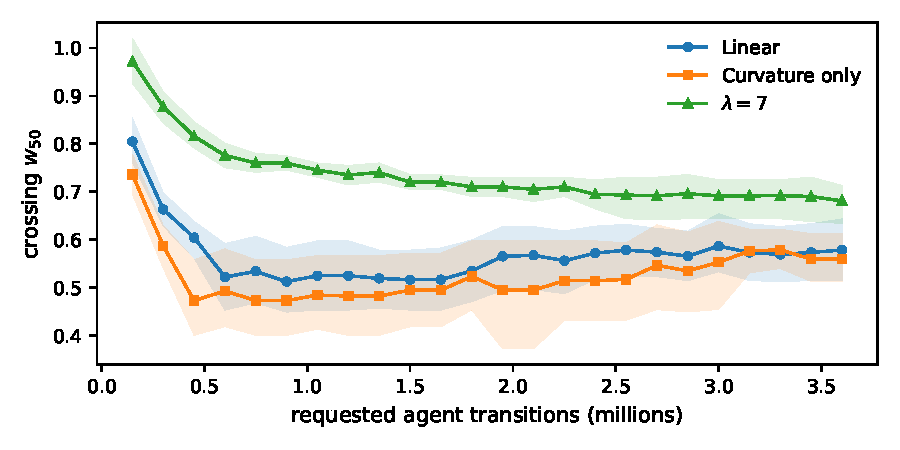
\includegraphics[width=.78\textwidth]{generated/v4/horizon_curves.pdf}
\caption{E3 crossings at every checkpoint (lines) with pointwise 95\% seed-block bands. Default optimizer; nine mixture cells, ten seeds per cell and condition.}
\label{fig:horizon}
\Description{Three crossing curves over training budget: lambda seven decreasing throughout; linear and curvature-only falling to 900k and rising afterwards.}
\end{figure}
\FloatBarrier

\section{Optimizer Factorial Details}
\label{app:factorial}

\begin{table}[H]
\caption{Change in each contrast relative to the default cell (global clip, raw reward), paired by seed. $^{\ast}$: interval excludes zero.}
\label{tab:factorial_interactions}
\centering\footnotesize
\begin{tabular}{@{}lcccc@{}}
\toprule
Intervention & $\Delta$(A$-$S) & $\Delta$(A$-$B) & $\Delta$(S$-$B) & $\Delta$(R$-$B) \\
\midrule
Global clip, normalized reward & \begin{tabular}[t]{@{}c@{}}$+0.311$$^{\ast}$\\[-1pt]{\scriptsize $[+0.220,\,+0.402]$}\end{tabular} & \begin{tabular}[t]{@{}c@{}}$+0.003$\\[-1pt]{\scriptsize $[-0.130,\,+0.146]$}\end{tabular} & \begin{tabular}[t]{@{}c@{}}$-0.308$$^{\ast}$\\[-1pt]{\scriptsize $[-0.443,\,-0.158]$}\end{tabular} & \begin{tabular}[t]{@{}c@{}}$-0.195$$^{\ast}$\\[-1pt]{\scriptsize $[-0.349,\,-0.046]$}\end{tabular} \\
Separate optimizers, raw & \begin{tabular}[t]{@{}c@{}}$+0.248$$^{\ast}$\\[-1pt]{\scriptsize $[+0.136,\,+0.373]$}\end{tabular} & \begin{tabular}[t]{@{}c@{}}$+0.051$\\[-1pt]{\scriptsize $[-0.071,\,+0.161]$}\end{tabular} & \begin{tabular}[t]{@{}c@{}}$-0.197$$^{\ast}$\\[-1pt]{\scriptsize $[-0.366,\,-0.021]$}\end{tabular} & \begin{tabular}[t]{@{}c@{}}$-0.229$$^{\ast}$\\[-1pt]{\scriptsize $[-0.350,\,-0.104]$}\end{tabular} \\
Separate optimizers, normalized & \begin{tabular}[t]{@{}c@{}}$+0.311$$^{\ast}$\\[-1pt]{\scriptsize $[+0.209,\,+0.396]$}\end{tabular} & \begin{tabular}[t]{@{}c@{}}$-0.096$\\[-1pt]{\scriptsize $[-0.239,\,+0.034]$}\end{tabular} & \begin{tabular}[t]{@{}c@{}}$-0.407$$^{\ast}$\\[-1pt]{\scriptsize $[-0.565,\,-0.258]$}\end{tabular} & \begin{tabular}[t]{@{}c@{}}$-0.320$$^{\ast}$\\[-1pt]{\scriptsize $[-0.480,\,-0.174]$}\end{tabular} \\
Global clip, raw, Adam $\epsilon{=}10^{-8}$ & \begin{tabular}[t]{@{}c@{}}$+0.122$$^{\ast}$\\[-1pt]{\scriptsize $[+0.008,\,+0.253]$}\end{tabular} & \begin{tabular}[t]{@{}c@{}}$+0.023$\\[-1pt]{\scriptsize $[-0.087,\,+0.132]$}\end{tabular} & \begin{tabular}[t]{@{}c@{}}$-0.099$\\[-1pt]{\scriptsize $[-0.243,\,+0.033]$}\end{tabular} & \begin{tabular}[t]{@{}c@{}}$-0.090$\\[-1pt]{\scriptsize $[-0.201,\,+0.036]$}\end{tabular} \\
\bottomrule
\end{tabular}
\end{table}

\begin{table}[t]
\caption{Optimizer diagnostics (means over runs of per-minibatch means). Pre-clip critic and actor gradient norms, post-clip (applied) actor norm, actor share of squared gradient norm, fraction of minibatches whose norm exceeds 0.5, and transformed-reward RMS. With separate optimizers no clipping is applied, so the applied actor norm equals the pre-clip norm.}
\label{tab:factorial_diagnostics}
\centering\scriptsize
\resizebox{\linewidth}{!}{%
\begin{tabular}{@{}llrrrrrr@{}}
\toprule
Cell & Arm & Critic & Actor & Applied actor & Actor share & Over 0.5 & Reward RMS \\
\midrule
Global clip, raw (default) & B & 1,326.81 & 2.07 & 0.0015 & 0.000 & 1.000 & 8.7 \\
 & A & 3,425.24 & 1.83 & 0.0009 & 0.000 & 1.000 & 30.1 \\
 & S & 11,964.76 & 1.46 & 0.0002 & 0.000 & 1.000 & 56.9 \\
Global clip, normalized reward & B & 0.12 & 4.39 & 0.4967 & 0.989 & 0.999 & 9.9 \\
 & A & 0.14 & 4.22 & 0.4962 & 0.988 & 0.999 & 31.4 \\
 & S & 0.12 & 4.25 & 0.4966 & 0.989 & 0.999 & 68.9 \\
Separate optimizers, raw & B & 1,285.95 & 4.06 & 4.0562 & 0.000 & 1.000 & 9.8 \\
 & A & 3,737.64 & 3.63 & 3.6322 & 0.000 & 1.000 & 30.6 \\
 & S & 13,923.98 & 4.41 & 4.4090 & 0.000 & 1.000 & 64.1 \\
Separate optimizers, normalized & B & 0.12 & 3.86 & 3.8594 & 0.986 & 0.999 & 9.8 \\
 & A & 0.14 & 3.86 & 3.8567 & 0.985 & 0.999 & 31.5 \\
 & S & 0.12 & 3.99 & 3.9904 & 0.987 & 0.999 & 69.5 \\
Global clip, raw, Adam $\epsilon{=}10^{-8}$ & B & 1,286.02 & 2.70 & 0.0019 & 0.000 & 1.000 & 9.0 \\
 & A & 3,828.34 & 2.43 & 0.0011 & 0.000 & 1.000 & 31.1 \\
 & S & 11,698.56 & 2.42 & 0.0003 & 0.000 & 1.000 & 59.5 \\
\bottomrule
\end{tabular}
}
\end{table}

\begin{table}[H]
\caption{E1/E2 observed collapsed runs out of ten seeds per mixture cell at 300k.}
\label{tab:factorial_cells}
\centering\scriptsize
\begin{tabular}{@{}llrrrrrrrr@{}}
\toprule
Cell & Arm & $w{=}0$ & $w{=}0.2$ & $w{=}0.4$ & $w{=}0.5$ & $w{=}0.6$ & $w{=}0.7$ & $w{=}0.85$ & $w{=}1$ \\
\midrule
Global clip, raw (default) & B & 10 & 10 & 9 & 5 & 4 & 1 & 0 & 0 \\
 & A & 10 & 10 & 10 & 10 & 10 & 10 & 3 & 0 \\
 & S & 10 & 10 & 10 & 10 & 10 & 10 & 7 & 1 \\
 & R & 10 & 10 & 10 & 10 & 10 & 10 & 1 & 0 \\
Global clip, normalized reward & B & 10 & 6 & 4 & 2 & 0 & 0 & 0 & 0 \\
 & A & 10 & 10 & 9 & 8 & 4 & 3 & 0 & 0 \\
 & S & 10 & 8 & 4 & 2 & 1 & 0 & 0 & 0 \\
 & R & 10 & 10 & 3 & 1 & 0 & 0 & 0 & 0 \\
Separate optimizers, raw & B & 10 & 9 & 2 & 1 & 0 & 0 & 0 & 0 \\
 & A & 10 & 10 & 10 & 10 & 9 & 2 & 0 & 0 \\
 & S & 10 & 10 & 7 & 3 & 4 & 0 & 1 & 0 \\
 & R & 10 & 9 & 3 & 2 & 0 & 0 & 0 & 0 \\
Separate optimizers, normalized & B & 10 & 10 & 5 & 2 & 1 & 0 & 1 & 0 \\
 & A & 10 & 10 & 10 & 9 & 4 & 2 & 0 & 0 \\
 & S & 10 & 8 & 6 & 1 & 0 & 0 & 0 & 0 \\
 & R & 10 & 8 & 5 & 1 & 0 & 0 & 0 & 0 \\
Global clip, raw, Adam $\epsilon{=}10^{-8}$ & B & 10 & 10 & 5 & 4 & 1 & 2 & 0 & 0 \\
 & A & 10 & 10 & 10 & 10 & 10 & 9 & 0 & 0 \\
 & S & 10 & 10 & 10 & 9 & 9 & 4 & 2 & 0 \\
 & R & 10 & 10 & 10 & 6 & 7 & 3 & 0 & 0 \\
\bottomrule
\end{tabular}
\end{table}

\begin{table}[H]
\caption{Fraction of training rewards on the loss branch ($x-z_0<0$, $z_0=-2.628$), by mixture weight, for the default and the fully decoupled E1 cells. The fraction depends on $w$ and on the learned policy; near the crossings both branches are active.}
\label{tab:loss_occupancy}
\centering\scriptsize
\begin{tabular}{@{}llrrrrrrrr@{}}
\toprule
Cell & Arm & $w{=}0$ & $w{=}0.2$ & $w{=}0.4$ & $w{=}0.5$ & $w{=}0.6$ & $w{=}0.7$ & $w{=}0.85$ & $w{=}1$ \\
\midrule
Global clip, raw (default) & B & 0.59 & 0.63 & 0.50 & 0.37 & 0.26 & 0.18 & 0.10 & 0.08 \\
 & A & 0.59 & 0.65 & 0.58 & 0.57 & 0.55 & 0.49 & 0.13 & 0.07 \\
 & S & 0.59 & 0.64 & 0.57 & 0.54 & 0.48 & 0.37 & 0.17 & 0.08 \\
Separate optimizers, normalized & B & 0.58 & 0.58 & 0.32 & 0.18 & 0.14 & 0.10 & 0.08 & 0.07 \\
 & A & 0.58 & 0.62 & 0.51 & 0.38 & 0.24 & 0.17 & 0.09 & 0.08 \\
 & S & 0.58 & 0.52 & 0.24 & 0.19 & 0.14 & 0.11 & 0.09 & 0.07 \\
\bottomrule
\end{tabular}
\end{table}


\begin{figure}[H]
\centering
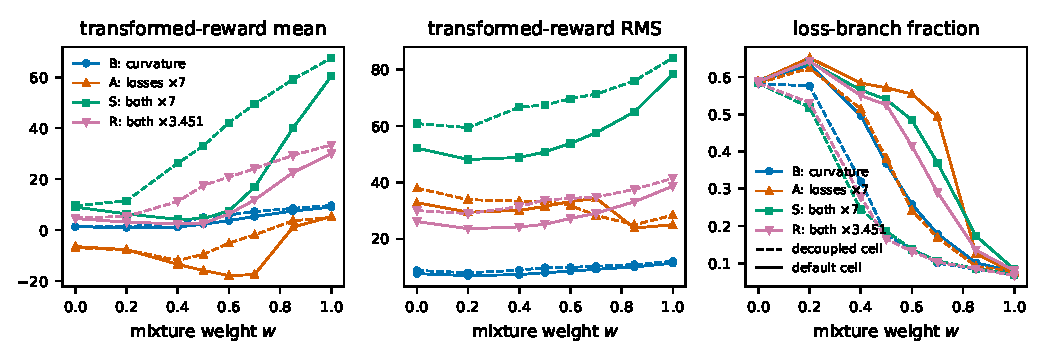
\includegraphics[width=\textwidth]{generated/v4/fig_reward_moments.pdf}
\caption{Transformed-reward moments over training in E1, by arm and mixture weight: mean, RMS and fraction on the loss branch (per-run means, averaged over seeds), for the default cell (solid) and the fully decoupled cell (dashed). The per-run tables keep these moments; per-rollout quantiles were also logged and are summarized for E7 in Table~\ref{tab:dist}.}
\label{fig:reward_moments}
\Description{Three line panels against mixture weight; A has a negative mean while S and R have growing positive means; RMS is largest for S.}
\end{figure}

\begin{figure}[H]
\centering
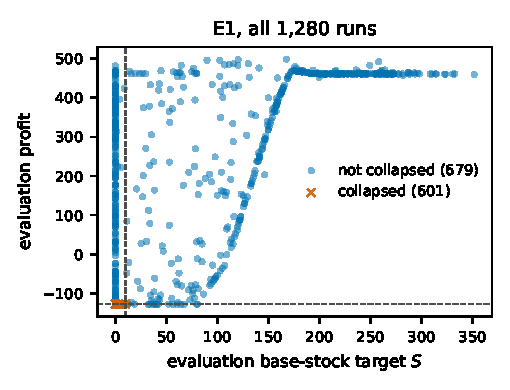
\includegraphics[width=.5\textwidth]{generated/v4/fig_label.pdf}
\caption{Collapse-label validation on all E1 runs: evaluation base-stock target $\bar S$ against evaluation profit, with the two label thresholds ($\bar S<10$, profit $\le-127.1$) dashed. Collapsed runs sit at the lazy-policy corner.}
\label{fig:label}
\Description{Scatter of profit against base-stock target; collapsed runs cluster at near-zero target and profit near minus 128.}
\end{figure}
\FloatBarrier

\begin{table}[H]
\caption{E7 training-reward and critic-target distributions. Per-rollout statistics of the transformed training reward (pooled over the five nodes) and of the rollout-buffer returns that the critic regresses, averaged over the 469 rollouts of each run and then over the 80 runs of each arm (ten seeds, eight cells). Quantile skewness is $(p_{90}+p_{10}-2p_{50})/(p_{90}-p_{10})$. M's reward statistics are reconstructed exactly from the logged B reward and M's frozen affine map; its fraction of negative rewards is not recoverable from the logs. Descriptive; not pre-registered.}
\label{tab:dist}
\centering\scriptsize\setlength{\tabcolsep}{4pt}
\begin{tabular}{@{}llrrrrrrrrr@{}}
\toprule
& & \multicolumn{7}{c}{Training reward (per rollout)} & \multicolumn{2}{c}{Critic targets} \\
\cmidrule(lr){3-9}\cmidrule(l){10-11}
Critic & Arm & Mean & SD & $p_{10}$ & $p_{50}$ & $p_{90}$ & Q-skew & Frac.\ $<0$ & Mean & SD \\
\midrule
Plain & B (curvature) & $+5.5$ & 7.0 & $-1.0$ & $+5.8$ & $+13.0$ & $+0.01$ & 0.23 & $+68$ & 50 \\
Plain & A (losses $\times7$) & $-6.6$ & 22.4 & $-25.7$ & $-3.9$ & $+12.2$ & $-0.12$ & 0.40 & $-104$ & 113 \\
Plain & S (both $\times7$) & $+31.5$ & 47.5 & $-15.1$ & $+31.0$ & $+88.9$ & $+0.10$ & 0.30 & $+256$ & 270 \\
Plain & M (affine of B) & $-13.5$ & 26.2 & $-38.9$ & $-15.4$ & $+20.0$ & $+0.18$ & -- & $-185$ & 148 \\
PopArt & B (curvature) & $+5.5$ & 7.0 & $-1.2$ & $+5.9$ & $+13.0$ & $-0.01$ & 0.23 & $+73$ & 53 \\
PopArt & A (losses $\times7$) & $-3.1$ & 22.2 & $-21.0$ & $+1.5$ & $+12.6$ & $-0.27$ & 0.32 & $-70$ & 123 \\
PopArt & S (both $\times7$) & $+38.5$ & 48.6 & $-7.8$ & $+40.4$ & $+91.0$ & $+0.01$ & 0.24 & $+501$ & 371 \\
PopArt & M (affine of B) & $-4.8$ & 26.3 & $-29.2$ & $-3.9$ & $+22.4$ & $-0.02$ & -- & $-90$ & 146 \\
\bottomrule
\end{tabular}
\end{table}

\FloatBarrier

\section{Level-Based Foraging Details}
\label{app:lbf}

\begin{table}[H]
\caption{E4 observed collapsed runs out of ten seeds per mixture cell (2M timesteps).}
\label{tab:lbf_cells}
\centering\scriptsize
\begin{tabular}{@{}llrrrrrrrrrr@{}}
\toprule
Optimizer & Arm & $w{=}0$ & $w{=}0.1$ & $w{=}0.2$ & $w{=}0.3$ & $w{=}0.5$ & $w{=}0.65$ & $w{=}0.75$ & $w{=}0.85$ & $w{=}0.9$ & $w{=}0.95$ \\
\midrule
Global clip & Linear & 4 & 1 & 1 & 3 & 0 & 0 & 1 & 0 & 0 & 0 \\
 & Curvature & 9 & 9 & 3 & 2 & 2 & 2 & 0 & 0 & 0 & 0 \\
 & A ($\lambda{=}4$) & 9 & 9 & 9 & 9 & 9 & 8 & 9 & 4 & 2 & 0 \\
 & S ($\times4$) & 9 & 8 & 7 & 4 & 5 & 1 & 0 & 0 & 0 & 0 \\
Separate, no clip & Linear & 7 & 6 & 0 & 2 & 1 & 0 & 0 & 0 & 0 & 0 \\
 & Curvature & 6 & 9 & 7 & 2 & 2 & 1 & 0 & 0 & 0 & 0 \\
 & A ($\lambda{=}4$) & 9 & 9 & 9 & 9 & 9 & 9 & 9 & 4 & 5 & 0 \\
 & S ($\times4$) & 9 & 8 & 8 & 5 & 6 & 0 & 0 & 0 & 0 & 0 \\
\bottomrule
\end{tabular}
\end{table}

\begin{table}[H]
\caption{E4 sensitivity to the collapse threshold $\theta$ (native team return) and to the estimator. The stored run labels used $\theta=0.5$ (deviation D4); the pre-declared $\theta=0.626$ is primary. Last column: difference of decreasing-isotonic crossings.}
\label{tab:lbf_theta}
\centering\footnotesize
\begin{tabular}{@{}llcccc@{}}
\toprule
$\theta$ & Optimizer & A & S & A$-$S (Firth) & A$-$S (isotonic) \\
\midrule
0.500 & Global clip & \begin{tabular}[t]{@{}c@{}}$0.525$\\[-1pt]{\scriptsize $[0.188,\,0.719]$}\end{tabular} & \begin{tabular}[t]{@{}c@{}}$0.107$\\[-1pt]{\scriptsize $[-0.065,\,0.225]$}\end{tabular} & \begin{tabular}[t]{@{}c@{}}$+0.418$\\[-1pt]{\scriptsize $[+0.218,\,+0.553]$}\end{tabular} & $+0.575$ \\
 & Separate, no clip & \begin{tabular}[t]{@{}c@{}}$0.557$\\[-1pt]{\scriptsize $[0.250,\,0.724]$}\end{tabular} & \begin{tabular}[t]{@{}c@{}}$0.077$\\[-1pt]{\scriptsize $[-0.126,\,0.237]$}\end{tabular} & \begin{tabular}[t]{@{}c@{}}$+0.479$\\[-1pt]{\scriptsize $[+0.289,\,+0.613]$}\end{tabular} & $+0.731$ \\
0.626 & Global clip & \begin{tabular}[t]{@{}c@{}}$0.771$\\[-1pt]{\scriptsize $[0.584,\,0.876]$}\end{tabular} & \begin{tabular}[t]{@{}c@{}}$0.324$\\[-1pt]{\scriptsize $[0.179,\,0.451]$}\end{tabular} & \begin{tabular}[t]{@{}c@{}}$+0.447$\\[-1pt]{\scriptsize $[+0.312,\,+0.559]$}\end{tabular} & $+0.548$ \\
 & Separate, no clip & \begin{tabular}[t]{@{}c@{}}$0.843$\\[-1pt]{\scriptsize $[0.623,\,0.918]$}\end{tabular} & \begin{tabular}[t]{@{}c@{}}$0.353$\\[-1pt]{\scriptsize $[0.224,\,0.468]$}\end{tabular} & \begin{tabular}[t]{@{}c@{}}$+0.490$\\[-1pt]{\scriptsize $[+0.315,\,+0.619]$}\end{tabular} & $+0.325$ \\
0.750 & Global clip & \begin{tabular}[t]{@{}c@{}}$0.889$\\[-1pt]{\scriptsize $[0.812,\,1.198]$}\end{tabular} & \begin{tabular}[t]{@{}c@{}}$0.519$\\[-1pt]{\scriptsize $[0.394,\,0.610]$}\end{tabular} & \begin{tabular}[t]{@{}c@{}}$+0.370$\\[-1pt]{\scriptsize $[+0.259,\,+0.761]$}\end{tabular} & $+0.213$ \\
 & Separate, no clip & \begin{tabular}[t]{@{}c@{}}$0.921$\\[-1pt]{\scriptsize $[0.856,\,1.097]$}\end{tabular} & \begin{tabular}[t]{@{}c@{}}$0.474$\\[-1pt]{\scriptsize $[0.364,\,0.582]$}\end{tabular} & \begin{tabular}[t]{@{}c@{}}$+0.447$\\[-1pt]{\scriptsize $[+0.296,\,+0.694]$}\end{tabular} & $+0.354$ \\
\bottomrule
\end{tabular}
\end{table}

\begin{table}[H]
\caption{E4 fraction of training rewards below zero (reached through the LOAD effort cost), by mixture weight. Under A, agents largely stop attempting loads.}
\label{tab:lbf_occupancy}
\centering\scriptsize
\begin{tabular}{@{}llrrrrrrrrrr@{}}
\toprule
Optimizer & Arm & $w{=}0$ & $w{=}0.1$ & $w{=}0.2$ & $w{=}0.3$ & $w{=}0.5$ & $w{=}0.65$ & $w{=}0.75$ & $w{=}0.85$ & $w{=}0.9$ & $w{=}0.95$ \\
\midrule
Global clip & A ($\lambda{=}4$) & 0.012 & 0.014 & 0.013 & 0.014 & 0.018 & 0.020 & 0.021 & 0.042 & 0.059 & 0.112 \\
 & S ($\times4$) & 0.039 & 0.035 & 0.045 & 0.055 & 0.094 & 0.117 & 0.134 & 0.128 & 0.149 & 0.158 \\
 & Curvature & 0.045 & 0.051 & 0.069 & 0.085 & 0.086 & 0.115 & 0.133 & 0.138 & 0.131 & 0.153 \\
 & Linear & 0.089 & 0.100 & 0.105 & 0.141 & 0.165 & 0.176 & 0.169 & 0.166 & 0.165 & 0.176 \\
Separate, no clip & A ($\lambda{=}4$) & 0.012 & 0.012 & 0.012 & 0.012 & 0.013 & 0.015 & 0.017 & 0.040 & 0.046 & 0.100 \\
 & S ($\times4$) & 0.034 & 0.039 & 0.042 & 0.054 & 0.070 & 0.120 & 0.130 & 0.123 & 0.133 & 0.160 \\
 & Curvature & 0.042 & 0.042 & 0.054 & 0.075 & 0.096 & 0.108 & 0.122 & 0.132 & 0.143 & 0.143 \\
 & Linear & 0.066 & 0.076 & 0.118 & 0.137 & 0.161 & 0.172 & 0.169 & 0.162 & 0.157 & 0.175 \\
\bottomrule
\end{tabular}
\end{table}

\FloatBarrier

\section{Computational Accounting}
\label{app:compute}

E1--E8 comprise \VfourTrajectories{} trajectories and about \VfourCoreHours{} single-core hours
(Table~\ref{tab:compute_v4}), excluding smoke tests, equality gates and extraction. The legacy sweeps and
the earlier confirmation cohorts were run separately on another platform and are not included.

\begin{table}[H]
\caption{Measured v4 compute: completed Slurm array tasks, one CPU core each (single-thread PyTorch), summed elapsed time. Runs were executed at most eight concurrently.}
\label{tab:compute_v4}
\centering\small
\begin{tabular}{@{}llrrr@{}}
\toprule
ID & Experiment & Trajectories & Core-hours & Mean minutes per run \\
\midrule
E1 & Optimizer $\times$ normalization factorial, 300k & 1,280 & 177.5 & 8.3 \\
E2 & Adam-$\epsilon$ addendum, 300k & 320 & 44.4 & 8.3 \\
E3 & Refined horizon cohort to 3.6M & 270 & 449.4 & 99.9 \\
E4 & MAPPO on LBF, 2M timesteps & 800 & 143.2 & 10.7 \\
E5 & Decoupled horizon cohort to 3.6M & 270 & 450.4 & 100.1 \\
E6 & Clipping isolation, 300k & 720 & 101.4 & 8.4 \\
E7 & Critic-target normalization and moment control, 300k & 400 & 56.0 & 8.4 \\
E8 & Online moment control; fresh-seed replication, 300k & 480 & 67.1 & 8.4 \\
 & Total & 4,540 & 1,489.4 &  \\
\bottomrule
\end{tabular}
\end{table}

\FloatBarrier

\section{Reproducibility Artifact}
\label{app:artifact}

The anonymized archive, provided as supplementary material with this submission, contains the manuscript source; the frozen designs, pre-registration, hashes and
deviation log; the executed source for E1--E8; per-run tables for every E1--E8 trajectory (protocol,
label, evaluation summary and optimizer diagnostics); the extraction and analysis scripts; and the
renderer that produces every v4 table, figure and number. Labels are never taken from a stored field without
check: one module (\texttt{analysis/labels.py}) recomputes them from stored evaluation statistics, asserts each
declared threshold against the sentence of the pre-registration that declares it, rejects undeclared thresholds
and out-of-range inputs, and verifies that every stored supply-chain label equals the declared rule; unit tests
cover these checks and the E4 relabelling counts. Retraining every
trajectory is not part of the one-command rebuild: it regenerates all analyses, tables, figures and the PDF from
the per-run tables, and the executed source and frozen designs allow any run to be repeated. Raw per-minibatch diagnostics and checkpoints
(about 45\,GB) are available on request. The legacy sweeps are accompanied by their per-run records,
without a preserved execution environment.
